\documentclass[12pt,a4paper]{amsart}
\usepackage[slovene]{babel}
%\usepackage[cp1250]{inputenc}
\usepackage[T1]{fontenc}
\usepackage[utf8]{inputenc}
\usepackage{amsmath,amssymb,amsfonts}
\usepackage{url}
\usepackage[normalem]{ulem}
\usepackage[dvipsnames,usenames]{color}
\usepackage{graphicx}

% Oblika strani
\textwidth 15cm
\textheight 24cm
\oddsidemargin.5cm
\evensidemargin.5cm
\topmargin-5mm
\addtolength{\footskip}{10pt}
\pagestyle{plain}
\overfullrule=15pt % oznaci predlogo vrstico


% Ukazi za matematična okolja
\theoremstyle{definition} % tekst napisan pokončno
\newtheorem{definicija}{Definicija}[section]
\newtheorem{primer}[definicija]{Primer}
\newtheorem{opomba}[definicija]{Opomba}

\renewcommand\endprimer{\hfill$\diamondsuit$}


\theoremstyle{plain} % tekst napisan poševno
\newtheorem{lema}[definicija]{Lema}
\newtheorem{izrek}[definicija]{Izrek}
\newtheorem{trditev}[definicija]{Trditev}
\newtheorem{posledica}[definicija]{Posledica}


% Za številske mnozice uporabi naslednje simbole
\newcommand{\R}{\mathbb R}
\newcommand{\N}{\mathbb N}
\newcommand{\Z}{\mathbb Z}
\newcommand{\C}{\mathbb C}
\newcommand{\Q}{\mathbb Q}

% Ukaz za slovarsko geslo
\newlength{\odstavek}
\setlength{\odstavek}{\parindent}
\newcommand{\geslo}[2]{\noindent\textbf{#1}\hspace*{3mm}\hangindent=\parindent\hangafter=1 #2}


\newcommand{\program}{Finančna matematika} 
\newcommand{\imeavtorja}{Neža Kržan} 
\newcommand{\imementorja}{izr. prof. Jaka Smrekar} 
\newcommand{\naslovdela}{Statistika v kazenskem pravu}
\newcommand{\letnica}{2022} %letnica diplome


\begin{document}

%%%%%%%%%%%%%%%%%%%%%%%%%%%%%%%%%%%%%%%%%%%%%%%%%%%%%%%%%%%%%%%%%%%%%%%%%%%%%%%%%%%%%%%%%%%%%%%%%%%%%%%%%%%%%%%%%%%%%%%%%%%%%%%%%%%%%%%%%%%%
\thispagestyle{empty}
\noindent{\large
UNIVERZA V LJUBLJANI\\[1mm]
FAKULTETA ZA MATEMATIKO IN FIZIKO\\[5mm]
\program\ -- 1.~stopnja}
\vfill

\begin{center}{\large
\imeavtorja\\[2mm]
{\bf \naslovdela}\\[10mm]
Delo diplomskega seminarja\\[1cm]
Mentor: \imementorja}
\end{center}
\vfill

\noindent{\large
Ljubljana, \letnica}
\pagebreak

%%%%%%%%%%%%%%%%%%%%%%%%%%%%%%%%%%%%%%%%%%%%%%%%%%%%%%%%%%%%%%%%%%%%%%%%%%%%%%%%%%%%%%%%%%%%%%%%%%%%%%%%%%%%%%%%%%%%%%%%%%%%%%%%%%%%%%%%%%%%
\thispagestyle{empty}
\tableofcontents
\pagebreak

%%%%%%%%%%%%%%%%%%%%%%%%%%%%%%%%%%%%%%%%%%%%%%%%%%%%%%%%%%%%%%%%%%%%%%%%%%%%%%%%%%%%%%%%%%%%%%%%%%%%%%%%%%%%%%%%%%%%%%%%%%%%%%%%%%%%%%%%%%%%
%\thispagestyle{empty}
%\begin{center}
%{\bf \naslovdela}\\[3mm]
%{\sc Povzetek}
%\end{center}
% tekst povzetka v slovenscini
%V povzetku na kratko opišite vsebinske rezultate dela. Sem ne sodi razlaga organizacije dela -- v katerem poglavju/razdelku je kaj, pač pa le opis vsebine.
%\vfill
%\begin{center}
%{\bf Angle"ski naslov dela}\\[3mm] % prevod slovenskega naslova dela 
%{\sc Abstract}
%\end{center}
% tekst povzetka v anglescini
%Prevod zgornjega povzetka v angleščino.

%\vfill\noindent
%{\bf Math. Subj. Class. (2010):} navedite vsaj eno klasifikacijsko oznako -- dostopne so na \url{www.ams.org/mathscinet/msc/msc2010.html}  \\[1mm]  
%{\bf Ključne besede:} navedite nekaj ključnih pojmov, ki nastopajo v delu  \\[1mm]  
%{\bf Keywords:} angleški prevod ključnih besed
%\pagebreak

%%%%%%%%%%%%%%%%%%%%%%%%%%%%%%%%%%%%%%%%%%%%%%%%%%%%%%%%%%%%%%%%%%%%%%%%%%%%%%%%%%%%%%%%%%%%%%%%%%%%%%%%%%%%%%%%%%%%%%%%%%%%%%%%%%%%%%%%%%%%
%%%%%%%%%%%%%%%%%%%%%%%%%%%%%%%%%%%%%%%%%%%%%%%%%%%%%%%%%%%%%%%%%%%%%%%%%%%%%%%%%%%%%%%%%%%%%%%%%%%%%%%%%%%%%%%%%%%%%%%%%%%%%%%%%%%%%%%%%%%%
\section{Bayesova statistika}
Bayesova statistika je statistična veja, ki nam s pomočjo matematičnih pristopov omogoča uporabo verjetnosti pri reševanju statističnih 
problemov. V svoje modele vključuje pogojno verjetnost, katero izračunamo z uporabo Bayesovega pravila. \\

Zlasti Bayesovo sklepanje razlaga verjetnost kot merilo verjetnosti ali zaupanja, ki ga lahko ima posameznik glede nastanka določenega dogodka. 
O nekem dogodku lahko že imamo predhodno prepričanje oziroma apriorno prepričanje, ki pa se lahko spremeni, ko se pojavijo novi dokazi. Bayesova 
statistika nam daje matematične modele za vključevanje naših apriornih prepričanj in dokazov za ustvarjenje novih prepričanj oziroma za 
pridobitev aposteriornega prepričanja, ki se lahko uporabi za kasnejše odločitve.

%%%%%%%%%%%%%%%%%%%%%%%%%%%%%%%%%%%%%%%%%%%%%%%%%%%%%%%%%%%%%%%%%%%%%%%%%%%%%%%%%%%%%%%%%%%%%%%%%%%%%%%%%%%%%%%%%%%%%%%%%%%%%%%%%%%%%%%%%%%%
\subsection{Bayesovo pravilo} 
Bayesovo sklepanje temelji na Bayesovim pravilom, ki izraža verjetnost nekega dogodka z verjetnostjo dveh dogodkov in obrnejnje pogojne 
verjetnosti. Pogojna verjetnost predstavlja verjetnost dogodka, glede na drug dogodek. 

\begin{definicija}
Pogojna verjetnost dogodka H, glede na dogodek E, je
\begin{equation}\label{eq:pogojna}
P(H \lvert E) = \frac{P(H \cap E)}{P(E)},
\end{equation}
ob predpostavki, da je $P(E) > 0$.
\end{definicija}

Formula \eqref{eq:pogojna} pove, da je verjetnost dogodka H ob pogoju, da se je zgodil dogodek E, enaka razmerju verjetnosti, da se 
zgodita oba dogodka in verjetnosti, da se je zgodil dogodek E.\\

Potem pogojno verjetnost uporabimo še v števcu formule \eqref{eq:pogojna} in dobimo Bayesovo pravilo:
\begin{equation}\label{eq:bpravilo}
    P(H \lvert E) = \frac{P(E \lvert H) \times P(H)}{P(E)},
\end{equation}

verjetnost dogodka E lahko še razpišemo in dobimo:
\begin{equation}\label{eq:b_pravilo}
    P(H \lvert E) = \frac{P(E \lvert H) \times P(H)}{P(E \lvert H)P(H) + P(E \lvert \neg H)P(\neg H)}.
\end{equation} \\

Obstaja še ena formulacija Bayesovega pravila, ki olajša izračune in je pogosto uporabljena pri Bayesovi analizi DNK dokazov:
\begin{equation}\label{eq:b_pravilo_DNK}
    \frac{P(H \lvert E)}{P(\neg H \lvert E)} = \frac{P(E \lvert H)}{P(E \lvert \neg H)} \times \frac{P(H)}{P(\neg H)}.
\end{equation}\\

%%%%%%%%%%%%%%%%%%%%%%%%%%%%%%%%%%%%%%%%%%%%%%%%%%%%%%%%%%%%%%%%%%%%%%%%%%%%%%%%%%%%%%%%%%%%%%%%%%%%%%%%%%%%%%%%%%%%%%%%%%%%%%%%%%%%%%%%%%%%
\subsection{Bayesovo posodabljanje}
Bayesovo pravilo se razlikuje od Bayesovega posodabljanja. Prvo je matematični izrek, drugo pa logična trditev, kako se sčasoma posodabljajo 
apriorne verjetnosti dokazov glede na novo zbrane dokaze oziroma prepričanja. \\

Bayesovo posodabljanje pravi:
\begin{trditev}
Če se dogodek E zgodi ob času $t_1 > t_0$, potem je $P_1(H) = P_0(H \lvert E)$.
\end{trditev}

Ob času $t_0$ dogodku H dodelimo verjetnost $P_0(H)$; to se imenuje predhodna verjetnost oziroma apriorna verjetnost. Ko se zgodi dogodek E 
ob času $t_1$, ki vpliva na naša prepričanja o dogodku H, Bayesovo posodabljanje pravi, da je potrebno apriorno verjetnost dogodka H v času $t_1$ 
enačiti z pogojno verjetnostjo dogodka H glede na dogodek E v času $t_0$. \\

Recimo, da je dogodek H neka hipoteza oziroma prepričanje o zločinu in dogodek E dokazi, zbrani za ta zložin. Pri Bayesovem posodabljanju je videti, 
kot da je dokaz E nesporno resničen. Z drugimi besedami, predpostavka je, da moramo imeti po zbiranju dokazov E stopnjo zaupanja v E enako 1, 
torej če so dokazi zbarni v času $t_1$, je $P_1(E)=1$. \\\\

%%%%%%%%%%%%%%%%%%%%%%%%%%%%%%%%%%%%%%%%%%%%%%%%%%%%%%%%%%%%%%%%%%%%%%%%%%%%%%%%%%%%%%%%%%%%%%%%%%%%%%%%%%%%%%%%%%%%%%%%%%%%%%%%%%%%%%%%%%%%
%%%%%%%%%%%%%%%%%%%%%%%%%%%%%%%%%%%%%%%%%%%%%%%%%%%%%%%%%%%%%%%%%%%%%%%%%%%%%%%%%%%%%%%%%%%%%%%%%%%%%%%%%%%%%%%%%%%%%%%%%%%%%%%%%%%%%%%%%%%%
\section{Primer - Taksi podjetja}
Za lažje razumevanje Bayesovega pravila si poglejmo primer. \\

Obstajata dve taksi podjetji, Zeleni Taksi in Modri taksi, katerih vozila so pobarvana zeleno oziroma modro. Podjetje Zeleni taksi pokriva 
85 odstotokov trga, podjetje Modri taksi pa preostanek. Predpostavimo še, da v okolici ni drugih taksi podjetij. V meglenem dnevu taksi trči 
v mimoidočega pešca in ga poškoduje, vendar odpelje s kraja nesreče. Priča nesreče poroča, da je bilo vozilo modre barve. Priča ima prav le 
v 80 odstotokih primerov, kar pomeni, da je njegova zanesljivost enaka $0,8$. Kolikšna je verjetnost, da je bil taksi, ki je povzročil nesrečo, 
modre barve glede na poročilo priče? \\

Vpeljimo oznake:\\
$Z$ \dots hipoteza, da je bil taksi zelen, \\
$M$ \dots hipoteza, da je bil taksi moder, \\
$W_m$ \dots dokaz, t.j. poročanje priče, da je bil taksi moder. \\ \\
Problem je določiti pogojno verjetnost hipoteze $M$, ob pogoju, da je dokaz $W_m$ resničen, torej $P(M \lvert W_m)$. \\

Za uporabo Bayesovega pravila potrebujemo tri elemente: verjetnost dokazov glede na hipotezo, verjetnost dokazov in verjetnost hipoteze. Podjetje 
Zeleni taksi pokriva 85 odstotkov trga, zato je verjetnost $P(Z)=0,85$. Po definiciji verjetnosti, je potem $P(M)=1-P(Z)=0,15$. Vemo tudi, da ima 
priča v 80 odstotkih primerov prav, torej $P(W_m \lvert M) = 0,8$ in $P(W_m \lvert Z) = 0,2$. Izračunajmo še verjetnost dokaza $P(W_m)$:\\
\[P(W_m) = P(W_m \lvert B)P(M) + P(W_m \lvert Z)P(Z)= 0,8 \times 0,15 + 0,2 \times 0,85 = 0,29.\]\\

Sedaj lahko uporabimo Bayesovo pravilo:
\[P(M \lvert W_m)= \frac{P(W_m \lvert M)P(M)}{P(W_m \lvert M)P(M) + P(W_m \lvert Z)P(Z)} = \frac{0,8 \times 0,15}{0,29} = \frac{12}{29} \approx 0,41.\] \\

Verjetnost, da je bil taksi glede na pričanje dejansko modre barve, je precej majhna, tudi če ima priča v 80 odstotokih primerov prav. Razlog za to je, 
da je verjetnost $M$, ne glede na dokaze, majhna ($P(M)=0,15$). Spodnja tabela kaže, da lahko s spreminjanjem verjetnosti $M$ dobimo različne pogojne 
verjetnosti $P(M \lvert W_m)$, pri čemer je zanesljivost priče nespremenjena:

\begin{table}[h!]
\centering
\begin{tabular}{c c c c} 
\hline
$P(M)$ & $P(Z)$ & $P(W_m \lvert M)$ & $P(M \lvert W_m)$ \\ 
\hline
0,15 & 0,85 & 0,8 & 0,41 \\
0,25 & 0,75 & 0,8 & 0,57 \\
0,35 & 0,65 & 0,8 & 0,68 \\
0,45 & 0,55 & 0,8 & 0,76 \\
0,50 & 0,50 & 0,8 & 0,80 \\
0,55 & 0,45 & 0,8 & 0,83 \\
0,65 & 0,35 & 0,8 & 0,88 \\
0,75 & 0,25 & 0,8 & 0,92 \\
0,85 & 0,15 & 0,8 & 0,95 \\
\hline
\end{tabular} \vspace{3mm}
\end{table}
%%%%%%%%%%%%%%%%%%%%%%%%%%%%%%%%%%%%%%%%%%%%%%%%%%%%%%%%%%%%%%%%%%%%%%%%%%%%%%%%%%%%%%%%%%%%%%%%%%%%%%%%%%%%%%%%%%%%%%%%%%%%%%%%%%%%%%%%%%%%
%%%%%%%%%%%%%%%%%%%%%%%%%%%%%%%%%%%%%%%%%%%%%%%%%%%%%%%%%%%%%%%%%%%%%%%%%%%%%%%%%%%%%%%%%%%%%%%%%%%%%%%%%%%%%%%%%%%%%%%%%%%%%%%%%%%%%%%%%%%%
\section{Identifikacijski dokazi}
V kazenskih zadevah želimo vedeti, ali je obtoženec kriv ali ne. Če imamo torej na voljo dokaze $E$, nas zanima pogojna verjetnost 
$P(kriv \lvert E)$, pri čemer nam je lahko v pomoč Bayesovo pravilo. To v teoriji drži, čeprav je v praksi izračun verjetnostne krivde lahko 
preveč zapleten. Ampak z Bayesovim pravilom lahko ocenimo verjetnosti vmesnih trditev oziroma dokzaov, ki so ključnega pomena za ugotavljanje 
obtoženčeve krivde. Najbolj pogosta uporaba Bayesovega pravila je pri ugotavljanju, ali je obtoženec vir sledi DNK-ja s kraja zločina. \\

%%%%%%%%%%%%%%%%%%%%%%%%%%%%%%%%%%%%%%%%%%%%%%%%%%%%%%%%%%%%%%%%%%%%%%%%%%%%%%%%%%%%%%%%%%%%%%%%%%%%%%%%%%%%%%%%%%%%%%%%%%%%%%%%%%%%%%%%%%%%
\subsection{Poenostavljena Bayesova analiza}
Naj bo:\\
$S$ \dots trditev, da je obtoženec vir sledi DNK s kraja zločina; \\
$M$ \dots trditev, da se obtoženčev DNK ujema z DNK-jem s kraja zločina; \\
$f$ \dots funkcija pogostosti ujemanja DNK z DNK-jem s kraja zločina. \\
Želimo vedeti, kakšna je verjetnost S glede na M, tj. $P(S \lvert M)$. \\

Bayesovo pravilo lahko uporabimo na naslednji način:
\[\frac{P(S \lvert M)}{P(\neg S \lvert M)} = \frac{P(M \lvert S)}{P(M \lvert \neg S)} \times \frac{P(S)}{P(\neg S)}.\] \\
Verjetnosti $P(S)$ in $P(\neg S)$ je težko oceniti, ker ne vemo kakšna je množica osumljencev. Smiselno bi bilo, da zanju upoštevamo interval 
predhodnih verjetnosti in ocenimo njihov vpliv na ne verjetnost trditve $S$ in njene negacije. Nato moramo določiti vrednost $P(M \lvert S)$, ki 
je običajno enaka ena - če bi obtoženec dejansko pustil sledove, bi laboratorijske analize pokazale ujemanje(to imenujemo lažno 
negativni rezultat); to je sicer poenostavitev, saj se lahko zgodi, da analize ne pokažejo ujemanja, čeprav je obtoženec pustil sledi. 
Potrebujemo še verjetnost $P(M \lvert \neg S)$ (verjetnost, da se bo našlo ujemanje, če obtoženec ni vir sledi na kraju zločina). To je 
običajno enakovredno pogostosti ujemnja DNK-ja z DNK-jem s kraja zložina (tj. $f$);tudi to je poenostavitev, saj se lahko zgodi, da 
obtoženec nima enakega DNK profila, vendar so laboratorijske analize pokazale, da ga ima(to imenujemo lažno 
pozitivni rezultat).
Sledi:
\[\frac{P(S \lvert M)}{P(\neg S \lvert M)} = \frac{1}{f} \times \frac{P(S)}{P(\neg S)}.\] \\

%%%%%%%%%%%%%%%%%%%%%%%%%%%%%%%%%%%%%%%%%%%%%%%%%%%%%%%%%%%%%%%%%%%%%%%%%%%%%%%%%%%%%%%%%%%%%%%%%%%%%%%%%%%%%%%%%%%%%%%%%%%%%%%%%%%%%%%%%%%%
\subsection{Izpopolnjena Bayesova analiza}
Poenostavljena Bayesova analiza ne upošteva možnosti lažno pozitivne laboratorijske analize. Za upoštevanje te možnosti, bomo namesto $M$ 
uvedli spremenljivko $M_p$.\\
$M_p$ \dots poročano ujemanje laboratorijske analize; \\
$M_t$ \dots trditev, da obstaja dejansko ujemanje v DNK-ju;\\
$\neg M_t$ \dots teditev, da obstaja neujemanje v DNK-ju.  \\ 

Sledi: 
\[P(M_p \lvert \neg S) = P(M_p \lvert M_t)P(M_t \lvert \neg S) + P(M_p \lvert \neg M_t)P(\neg M_t \lvert \neg S). \vspace{3mm}\] 
Sedaj je $P(M_t \lvert \neg S)$ enako $f$ in zato $P(\neg M_t \lvert \neg S)$ enako $1-f$. $P(M_p \lvert \neg M_t)$ opisuje verjetnost lažno 
pozitivnih rezultatov laboratorija(oznaka $FP$) in $P(M_p \lvert M_t)$ verjetnost resničnih pozitivnih rezultatov laboratorija(oznaka $FN$). 
Sledi: \vspace{2mm}
\[P(M \lvert \neg S) = [(1 - FN) \times f] + [FP \times (1 - f)]. \vspace{3mm}\]

Formula pokaže, da za parvilno oceno verjetnosti $P(M_p \lvert \neg S)$ potrebujemo statistično oceno pogostosti profila DNK in stopnje napak 
laboratorijskih analiz, ki pa so redko na voljo. \vspace{3mm}

Druga poenostavitev je, da predpostavimo, da je $P(M_p \lvert S) = 1$, pri čemer ni upoštevana možnost lažnega negativnega rezultata. Kot zgoraj, imamo: \vspace{3mm}
\[P(M_p \lvert S) = P(M_p \lvert M_t)P(M_t \lvert S) + P(M_p \lvert \neg M_t)P(\neg M_t \lvert S). \vspace{3mm}\] 
Če je $P(M_p \lvert S) = 1$, je $P(\neg M_p \lvert S) = 0$ in $P(M_p \lvert S) = 1 - FN$. Potem sledi, da je: \vspace{3mm}
\[\frac{P(M_p \lvert S)}{P(M_p \lvert \neg S)} = \frac{1 - FN}{[(1 - FN) \times f] + [FN \times (1 - f)]}. \vspace{3mm}\]

Za predstavo, kako stopnje napak vplivajo na razmerje verjetnosti, predpostavim, da je pogostost profila DNK 1 proti milijardi. Predpostavim 
tudi, da sta stopnji lažno poztivnih in negativnih laboratorijskih rezuktatov(tj. FP in FN) enako $0,01$. Če je razmerje verjetnosti enako 
$\frac{1}{f}$, je milijarda. S formulo pa dobimo: \vspace{3mm}
\[\frac{P(M_p \lvert S)}{P(M_p \lvert \neg S)} = \frac{1 - 0,01}{[(1 - 0,01) \times 0,000000001] + [0,01 \times (1 - 0,000000001)]} \approx 99. \vspace{3mm}\]

Relativno majhne stopnje napak lahko bistveno zmanjšajo dokazno vrednost DNK dokazov, saj močno zmanjšajo rzmerje verjetnosti; v našem primeru 
smo iz milijarde prišli na pribljižno 100. \\\\

%%%%%%%%%%%%%%%%%%%%%%%%%%%%%%%%%%%%%%%%%%%%%%%%%%%%%%%%%%%%%%%%%%%%%%%%%%%%%%%%%%%%%%%%%%%%%%%%%%%%%%%%%%%%%%%%%%%%%%%%%%%%%%%%%%%%%%%%%%%%
%%%%%%%%%%%%%%%%%%%%%%%%%%%%%%%%%%%%%%%%%%%%%%%%%%%%%%%%%%%%%%%%%%%%%%%%%%%%%%%%%%%%%%%%%%%%%%%%%%%%%%%%%%%%%%%%%%%%%%%%%%%%%%%%%%%%%%%%%%%%
\section{Drugi pristopi}
Da bi ocenili moč Bayesove analize dokazov DNK, jo je koristno primerjati z nekaterimi drugimi pristopi. \\

%%%%%%%%%%%%%%%%%%%%%%%%%%%%%%%%%%%%%%%%%%%%%%%%%%%%%%%%%%%%%%%%%%%%%%%%%%%%%%%%%%%%%%%%%%%%%%%%%%%%%%%%%%%%%%%%%%%%%%%%%%%%%%%%%%%%%%%%%%%%
\subsection{Frekvence in edinstvenost}
Predlagano je bilo s strani mnogih avtorjev, da je bolj naraven način za obravnavo verjetnosti uporaba naravnih frekvenc(angl. natural 
frequencies). Recimo, da je pogostost profila DNK $f$ 1 proti 10 milijonov, predpostavimo tudi, da ima obtoženec enak DNK in da je začetna 
populacija osumljencev 100 milijonov ljudi. Zanima nas kakšna je verjetnost, da je obtoženec vir DNK-ja s kraja zločina. \\

Naj bo: \\
$f$ \dots pogostost profila DNK;\\
$m$ \dots velikost populacije osumljencev; \\
$n$ \dots število ljudi, ki imajo ustrezen DNK profil. \\
Po metodah, ki temeljijo na naravnih frekvencah, je potrebno izračunati, koliko ljudi z zadevnim profilom DNK je v populaciji osumljencem, tako 
da se $f$ pomnoži z $m$.  \\
Če je posameznikov s takim profilom $n > 1$, je verjetnost, da je obtoženi vir, $\frac{1}{n}$. V primeru, ko je $n < 1$ in so frekvence še 
posebaj majhne, je bolje raziskovati ali je profil DNK edinstven ali ne - ali poleg obtoženca obstajajo še drugi posamezniki z enakim 
profilom DNK. Temu pravimo metoda edinstvenosti(angl. uniqueness method). \\

S formulo binomske porazdelitve lahko izračunamo verjetnost, da se bo dogodek $X$, na primer profil DNK, pojavil $k$ - krat v $s$ - kratnem 
številu ponovitev, pri čemer ima dogodek $X$ frekvenco 4$f$. Želimo vedeti, kolikšna je verjetnost, da ima točno en posameznik ustrezen DNK 
profil, ob pogoju da ga ima vsaj en posameznik, torej: \vspace{3mm}
\[P(n = 1 \lvert n \ge 1) = \frac{P(n=1 \cap n \ge 1)}{P(n \ge 1)} = \frac{m \times f \times (1 - f)^{m-1}}{1 - (1-f)^m}. \vspace{3mm}\]

\begin{table}[h!]
    \centering
    \begin{tabular}{c c c c} 
    \hline
    $m$ & $f$ & $P(n = 1 \lvert n \ge 1)$ & $P(S \lvert M)$[Bayes]\\ 
    \hline
    10 milijonov & 1 v 100 milojonov & 0,9 & 0,9 \\
    100 milijonov & 1 v 100 milojonov & 0,62 & 0,5 \\
    1 milijarda & 1 v 100 milojonov & 0 & 0,09 \\ \hline
    10 milijonov & 1 v 1 milijardi & 1 & 0,99 \\
    100 milijonov & 1 v 1 milijardi & 0,9 & 0,9 \\
    1 milijarda & 1 v 1 milijardi & 0,62 & 0,5 \\ \hline
    10 milijonov & 1 v 10 milijardah & 1 & 0,999 \\
    100 milijonov & 1 v 10 milijardah & 1 & 0,99 \\
    1 milijarda & 1 v 10 milijardah & 0,9 & 0,9 \\ \hline
\end{tabular}
\end{table}

Tabela vsebuje primerjavo rezultatov, ki jih daje Bayesovo pravilo. Obe metodi se dokaj ujemata, vendar se tudi razlikujeta, saj v nasprotju 
z Bayesovim pravilom pri metodi edinstvenosti ni mogoče enostavno upoštevati številnih zapletov, kot je bil naprimer vpliv stopnje laboratorijskih napak. \\

%%%%%%%%%%%%%%%%%%%%%%%%%%%%%%%%%%%%%%%%%%%%%%%%%%%%%%%%%%%%%%%%%%%%%%%%%%%%%%%%%%%%%%%%%%%%%%%%%%%%%%%%%%%%%%%%%%%%%%%%%%%%%%%%%%%%%%%%%%%%
\subsection{Naključno ujemanje in razmerja verjetnosti}
Metoda verjetnost naključnega ujemanja(angl. random match probability) izraža možnost, da bi imel naključni posameznik, ki ni povezan z obdolžencem, 
ustrezni DNK profil. Ta verjetnost je enaka pogostosti profila DNK. Težava tega pristopa je, da verjetnost naključnega ujemanja lahko predstavljena 
oziroma razumevana narobe. \\

Pogosto se to verjetnost interpretira na slednji način:
\begin{enumerate}
    \item če je verjetnost naključnega ujemanja na primer 1 proti 100 milijonom, potem je verjetnost, da ima profil DNK drug posameznik in ne 
    obdolženec 1 proti 100 milijonom;
    \item ker je to zelo majhna verjetnost, mora biti tudi verjetnost, da je sled DNK pustil nekdo drug na kraju zločina in ne obdolženec, zelo majhna;
    \item zato mora biti verjetnost, da je vir sledi DNK s kraja zločina obtoženec zelo velika, ampak znaša 1 proti 100 milijonov.
\end{enumerate}
Takšno sklepanje je napašno in je znano kot tožilčeva zmota(angl. Prosecutor’s fallacy). Sestavlja jo enačba \vspace{3mm}
\begin{equation}\label{eq:tozilcevazmota}
    1 - f = P(S \lvert M).\vspace{3mm}
\end{equation}

Zmota se pojavi v koraku (2), ko je zamenjano $P(M \lvert \neg S)$ s $P(\neg S \lvert M)$ in predpostavljeno, da sta obe verjetnosti enaki $f$. \\

Namesto verjetnosti naključnega ujemanja forenzični strokovnjaki pogosto pričajo o razmerju verjetnosti(angl. likelihood ratio) dokazov DNK, in 
sicer kot: \vspace{3mm}
\[P(M \lvert S) = P(M \lvert \neg S). \vspace{3mm}\]
Bayesovo pravilo vključuje razmerje verjetnosti in predhodno oziroma pariorno verjetnost, torej je celovitejši način predstavitve dokazov DNK. 
Težavo ocenjevanja apriorne verjetnosti pri Bayesovem pravilu, bi lahko odpravili z osredotočanjem le na verjetnost. Metoda razmerja verjetnosi je 
koristna v državah kot sta naprimer Velika Britanija in Združene države Amerike, kjer se lahko Bayesovo pravilo šteje kot poseg v pravico porote 
do previdnosti: poroti naj ne bi bilo potrebno govoriti, kako naj razmišlja in presoja dokaze; Bayesovo pravilo pa je natanko metoda za 
tehtanje dokazov. \\\\

%%%%%%%%%%%%%%%%%%%%%%%%%%%%%%%%%%%%%%%%%%%%%%%%%%%%%%%%%%%%%%%%%%%%%%%%%%%%%%%%%%%%%%%%%%%%%%%%%%%%%%%%%%%%%%%%%%%%%%%%%%%%%%%%%%%%%%%%%%%%
%%%%%%%%%%%%%%%%%%%%%%%%%%%%%%%%%%%%%%%%%%%%%%%%%%%%%%%%%%%%%%%%%%%%%%%%%%%%%%%%%%%%%%%%%%%%%%%%%%%%%%%%%%%%%%%%%%%%%%%%%%%%%%%%%%%%%%%%%%%%
\section{Tožilčeva zmota}
Tožilčeva zmota(angl. Prosecutor’s fallacy) se pogosto pojavlja v kazenskem pravu, vendar jo pogosto neprepoznajo, deloma zato, ker preiskovalci 
nimajo močne intuicije o tem, kaj zmota sploh pomeni. Tožilčeva zmota je dobro znana statistična zmota, ki izhaja iz napačnega razumevanja 
pogojnih verjetnosti in vprašanj večkratnega testiranja. Napaka temelji na predpostavki, da je $P(H \lvert E) = P(E \lvert H)$, pri čemer $H$ 
predstavlja primer, da se najdejo dokazi o obtožencu, $E$ pa primer, da je obtoženec nedolžen. Vendar ta enakost ne drži: čeprav je $P(H \lvert E)$ 
običajno zelo majhen, je lahko $P(E \lvert H)$ še vedno veliko večji. \\

Za lažjo predstavo si oglejmo primer. Na primer, da ima storilec zločina enako krvno skupino kot obtoženec in da ima 10\% prebivalstva 
enako krvno skupino. Potem je lahko na podlagi tega verjetnost, da je obtoženec kriv, 90 odstotna. Vendar je ta sklep skoraj pravilen le, če 
je bil obtoženec izbran kot glavni osumljenec na podlagi trdnih dokazov, ki so bili odkriti pred krvnim testom in z njim nispo povezani, saj 
je lahko ujemanje krvi popolno naključje. V nasprotnem primeru je predstavljena utemeljitev napačna, saj ne upošteva predhodne verjetnosti, da 
gre za naključno nedolžno osebo. Denimo, da v mestu, kjer se je zgodil zločin, živi 1000 ljudi. To pomeni, da tam živi 100 ljudi, ki imajo 
krvno skupino storilca, zato je verjetnost, da je obtoženec kriv - na podlagi dejstva, da se njegova krvna skupina ujema s krvno skupino 
morilca - le 1\%, kar je veliko manj kot 90\%. \\

Do tožilčeve zmote lahko pride zaradi večkratnega testiranja, na primer pri primerjanju dokazov z veliko podatkovno bazo. Velikost podatkovne 
zbirke povečuje verjetnost, da bo ujemanje ugotovljeno zgolj po naključju. \\

Če je $E$ dokaz in $H$ trditev,da je obtoženi nedolžen, upoštevamo pogojne verjetnosti: \\
$P(E \lvert H)$ \dots verjetnost resničnosti dokaz $E$, kljub temu da je obtoženi nedolžen; \\
$P(H \lvert E)$ \dots verjetnodt, da je obtoženi nedolžen kljub dokazu $E$. \\
Pri forenzičnih dokazih je ponavadi verjetnost $P(E \lvert H)$ majhna. Tožilec pa potem velikokrat sklepa, da je tudi verjetnost 
$P(H \lvert E)$ majhna.
%(tožilstvo Lucie de Berk je na primer obtoženo ravno te napake)
Zgoraj napisani pogojni verjetnosti pa sta precej različni; uporabimo Bayesovo pravilo: \vspace{3mm}
\[P(H \lvert E) = P(E \lvert H) \times \frac{P(H)}{P(E)}, \vspace{3mm}\]
kjer je $P(H)$ verjetnost nedolžnosti in $P(E)$ verjetnost dokaza. Enačba kaže, da majhna pogojna verjetnost $P(E \lvert H)$ ne pomeni majhne 
pogojne verjetnosti $P(H \lvert E)$ v primeru velike verjetnosti nedolžnosti in majhne verjetnosti dokaza. \\

Po Bayesovem pravilu je \vspace{3mm}
\[P(E)=P(E \lvert H)P(H) + P(E \lvert \neg H)\times[1 - P(H)], \vspace{3mm}\]
kjer je $P(E \lvert \neg H)$ verjetnost, da bodo dokazi identificirali krivega osumljenca; bičajno je ta verjetnost blizu 1. 

%%%%%%%%%%%%%%%%%%%%%%%%%%%%%%%%%%%%%%%%%%%%%%%%%%%%%%%%%%%%%%%%%%%%%%%%%%%%%%%%%%%%%%%%%%%%%%%%%%%%%%%%%%%%%%%%%%%%%%%%%%%%%%%%%%%%%%%%%%%%
\subsection{Primer - Tožilčeva zmota}
Slika 1 prikazuje populacijo 100 moških, starih 50 let, ki se ne zdravijo zaradi hipertenzije in imajo skupni holesterol 235 mg/dl in krvni tlak 120 mmHg. Pričakuje
se, da bo 9\% teh moških (predstavljeno z devetimi črtastimi kvadrati) čez 10 let imelo miokardni infarkt(MI). Ena četrtina moških je kadilcev (predstavljeno s 25 
sivimi kvadrati); približno 16\% naj bi bilemo MI v 10 letih; zato bo $\frac{4}{25}$ kadilcev imelo MI (predstavljeno s črtastimi in sivimi kvadrati). \\
Število kadilcev, ki imajo MI, je očitno enako številu ljudi, ki imajo MI in so kadilci. Toda ali je delež kadilcev, ki imajo MI, enak deležu ljudi z MI, ki so kadilci? Iz 
slike 1 je odogovor očitno ne; verjetnost, da ste kadilec glede na to, da ste imeli MI, torej:
\[ P(\text{MI} \lvert \text{kadilec}) \ne P(\text{kadilec} \lvert \text{MI}), \quad \text{ker}\]
\[ P(\text{MI} \lvert \text{kadilec}) = P(\text{črtasto} \lvert \text{sivo}) = \frac{4}{25} = 0,16 \quad \text{in}\]
\[P(\text{kadilec} \lvert \text{MI}) = P(\text{sivo} \lvert \text{črtasto}) = \frac{4}{9} = 0,44.\]
Vizualno opazimo, da delež sivih kvadratov, ki se prekrivajo s črtastimi kvadrati, ni enak deležu črtastih kvadratov, ki se prekrivajo s sivimi kvadrati. 

\begin{figure}[!ht]\label{fig:slika1}
    \centering
    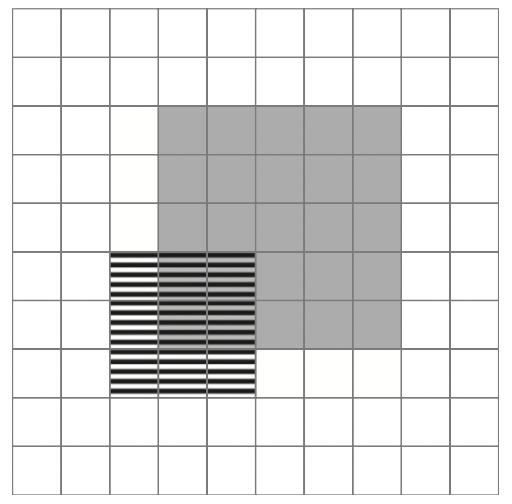
\includegraphics[scale=0.45]{slika1.png}
    \caption{Populacija, predstavljena s 100 kvadrati, z 9 črtastimi, 25 sivimi in 4 črtastimi in sivimi}\vspace{2mm}
 \end{figure}

 Slika 2 prikazuje izjeme pri tožilčevi zmoti, predstavljeni na sliki 1. Sedaj imamo 16 črtastih kvadratov, 16 sivih in 4 pikčaste in sive kvadrate, ker je splošna 
 razširjenost črtastih in sivih kvadratov enaka, je
 \[ P(\text{črtasto} \lvert \text{sivo}) = P(\text{sivo} \lvert \text{črtasto}).\]
Tudi 
\[P(\text{črtasto} \lvert \text{pikčasto}) = P(\text{pikčasto} \lvert \text{črtasto}),\]
saj sta obe verjetnosti enaki $0$. Oboje(podobno velike populacija in populacije brez prekrivanja) je ozka izjema zmote. \\
Po drugi strani pa so črtkani kvadrati na sliki 2 v celoti zajeti v sivih kvadratih; tako je 
\[P(\text{sivo} \lvert \text{črtkano}) = 1, \quad \text{medtem ko je} \quad P(\text{črtkano} \lvert \text{sivo}) = 0,25. \]
Tožilčeva zmota velja, kadar je ena skupina podmnožica druge.

\begin{figure}[!ht]\label{fig:slika2}
    \centering
    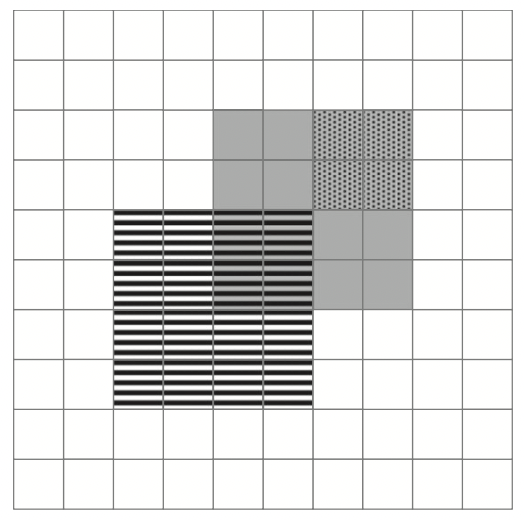
\includegraphics[scale=0.45]{slika2.png}
    \caption{Populacija, predstavljena s 100 kvadrati, z 16 črtastimi, 16 sivimi in 4 pikčastimi in sivimi}\vspace{2mm}
 \end{figure}
 
%%%%%%%%%%%%%%%%%%%%%%%%%%%%%%%%%%%%%%%%%%%%%%%%%%%%%%%%%%%%%%%%%%%%%%%%%%%%%%%%%%%%%%%%%%%%%%%%%%%%%%%%%%%%%%%%%%%%%%%%%%%%%%%%%%%%%%%%%%%%
%%%%%%%%%%%%%%%%%%%%%%%%%%%%%%%%%%%%%%%%%%%%%%%%%%%%%%%%%%%%%%%%%%%%%%%%%%%%%%%%%%%%%%%%%%%%%%%%%%%%%%%%%%%%%%%%%%%%%%%%%%%%%%%%%%%%%%%%%%%%
\section{Zmota obrambnega odvetnika}
Zmota zagovornika oziroma zmota obrambnega odvetnika(angl. Defense attorney's fallacy ) se pojavi, ko se poroča o tem, koliko ljudi z 
določeno značilnostjo, se pojavi v določeni populaciji. Predpostavlja se, da je storilec del neke poljubno velike populacije in da ni na voljo 
drugih informacij, torej je za vse enako verjetno, da so storilci. Na podlagi teh predpostavk lahko sklepamo, da obstaja majhna verjetnost, 
da je osumljenec storilec kaznivega dejanja. \\

%%%%%%%%%%%%%%%%%%%%%%%%%%%%%%%%%%%%%%%%%%%%%%%%%%%%%%%%%%%%%%%%%%%%%%%%%%%%%%%%%%%%%%%%%%%%%%%%%%%%%%%%%%%%%%%%%%%%%%%%%%%%%%%%%%%%%%%%%%%%
%%%%%%%%%%%%%%%%%%%%%%%%%%%%%%%%%%%%%%%%%%%%%%%%%%%%%%%%%%%%%%%%%%%%%%%%%%%%%%%%%%%%%%%%%%%%%%%%%%%%%%%%%%%%%%%%%%%%%%%%%%%%%%%%%%%%%%%%%%%%
% Seznam uporabljene literature
%https://www.quantstart.com/articles/Bayesian-Statistics-A-Beginners-Guide/
%https://en.wikipedia.org/wiki/Prosecutor%27s_fallacy 
%https://www.researchgate.net/publication/267131008_The_interrogator%27s_fallacy

\end{document}